% Provenance (never printed): see sources/outline_sources.md (Year 2: sedimentary basins;
% subsidence curves and backstripping; the stretching model). Stretching model after McKenzie
% (1978) as restated by Sheplev and Reverdatto (1998) and coded in pyBacktrack (EarthByte);
% backstripping after pyBacktrack's well module; North Sea after Sclater and Christie (1980);
% Michigan after Sloss (1982) and Crowe et al. (2009); the US Atlantic margin after Schlee et
% al. (1976), Poag (1979) and Lang et al. (2024); the Molasse after the chapter 13 rows.
% Curves and the invented well from figdata/bachelor-2/basins.py; exercise and problem values
% in the Book 4 scratch calculator calc/ch16.py.
\chapter{Cuencas sedimentarias comparadas}\label{ch:b2:basins-compared}

Frente a la costa del este de Estados Unidos, bajo la plataforma continental, la fosa de Baltimore
Canyon contiene al menos \qty{14}{km} de roca sedimentaria. Un sondeo perforado en una
pila así lee su historia al revés: cada unidad que atraviesa fue en su día el fondo marino, a una profundidad que
registran los fósiles y los sedimentos, y desde entonces ha sido enterrada y comprimida. La profundidad de cada
superficie datada es un punto de una curva de hundimiento. Sin embargo, la mayor parte del hundimiento la causó el
peso del propio sedimento. Para saber qué formó la cuenca hay que quitar ese peso,
capa a capa. Este capítulo muestra cómo, y lo que el resultado dice sobre la litosfera.
% ledger: poag79:bct, schlee76:atlantic

\begin{recall}
\textbf{Del volumen de primer año}: la cuenca sedimentaria, la subsidencia y la subsidencia tectónica,
el espacio de acomodación, la eustasia; la compactación, la descompactación y la ley de Athy, el espesor sólido de una
capa; la carga sedimentaria, que amplifica la subsidencia en un factor $(\rho_m - \rho_w)/(\rho_m - \rho_s)$;
la isostasia de Airy; la litosfera y su geoterma; los rifts continentales y los márgenes pasivos.
\textbf{De los volúmenes de física}: la ecuación del calor y sus soluciones de Fourier.
\textbf{Del \cref{ch:b2:alpine-orogen}}: la \omterm{def:b2:alpine-orogen:foreland}{cuenca de antepaís}, el \omterm{def:b2:alpine-orogen:foreland}{flysch} y la \omterm{def:b2:alpine-orogen:foreland}{molasa}.
\end{recall}

\begin{omfigure}
\centering
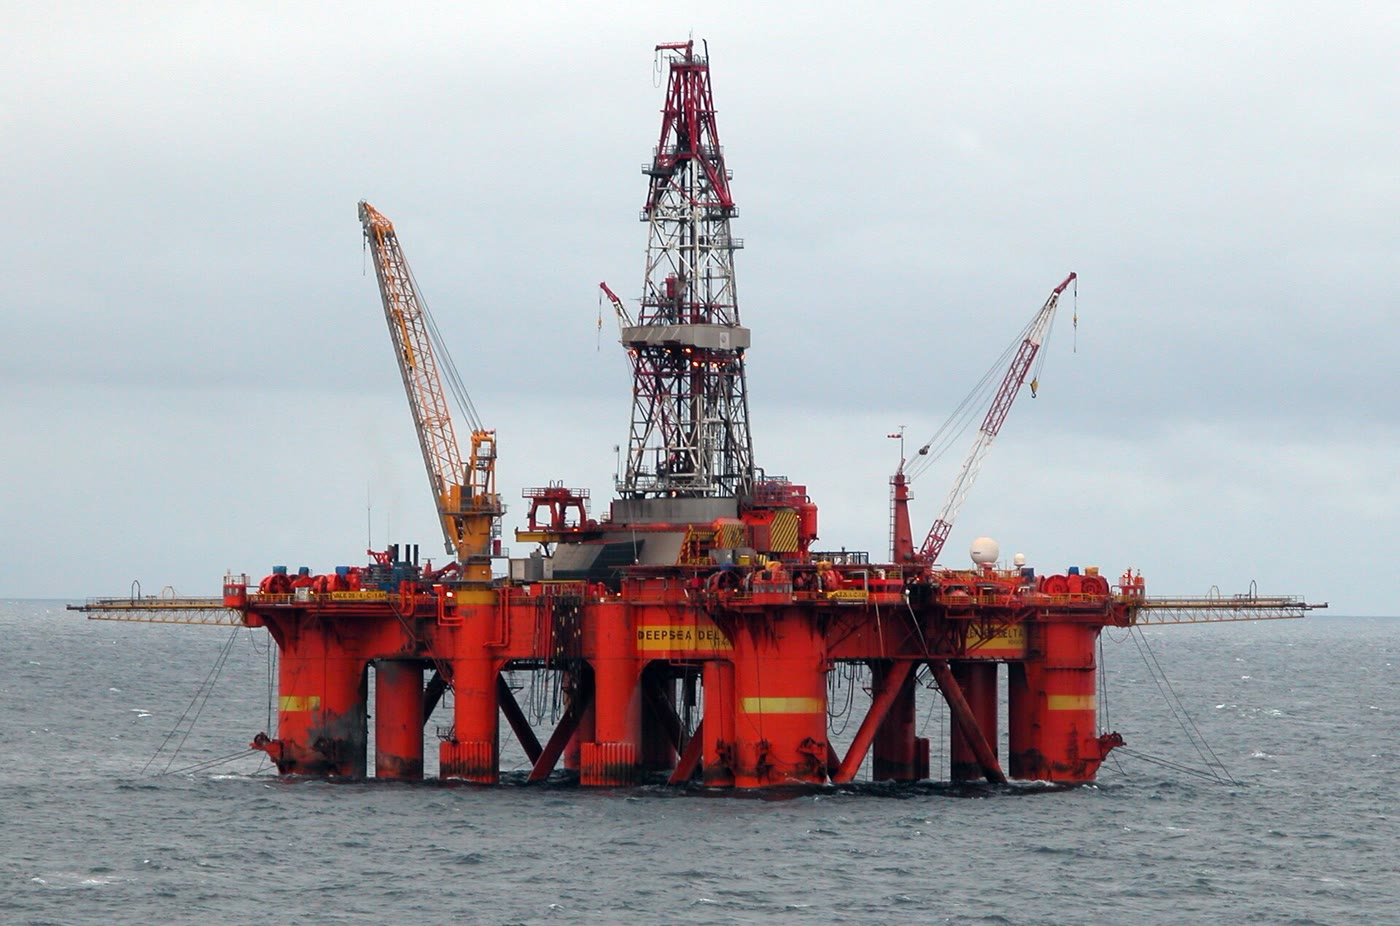
\includegraphics[width=0.66\linewidth]{images/book4/b2-16-drilling-rig.jpg}
\par\smallskip{\small Una plataforma de perforación semisumergible en el mar del Norte. Los sondeos perforados
desde estas plataformas dan los espesores, las edades y los tipos de roca a partir de los cuales se reconstruye la subsidencia
de una cuenca. Fotografía de Erik Christensen, 2005, CC BY-SA 3.0.}
\end{omfigure}

\section{Las cuencas y lo que las hace hundirse}\label{sec:b2:basins-compared:types}

El volumen de primer año distinguía las cuencas por el lugar donde se encuentran. Aquí se distinguen por lo que impulsa
su subsidencia.

\begin{definition}[Cuencas intracratónicas, de rift y de margen pasivo]\label{def:b2:basins-compared:types}
Una \emph{cuenca intracratónica}\index{cuenca intracratónica} es una cuenca amplia, redonda u ovalada, situada en el
interior de un continente, lejos de los límites de placa, que subside lentamente durante tiempos muy largos
sin fallas importantes. Una \emph{cuenca de rift}\index{cuenca de rift} es una cuenca limitada por fallas normales
en una litosfera continental sometida a estiramiento; su subsidencia sigue al estiramiento y después
al enfriamiento de la litosfera. Una \emph{cuenca de margen pasivo}\index{cuenca de margen pasivo} es la
cuña de sedimento, que se engruesa hacia el océano, acumulada sobre un margen continental tras la
ruptura, sobre la corteza adelgazada del antiguo rift.
\end{definition}

La \omterm{def:b2:alpine-orogen:foreland}{cuenca de antepaís} del \cref{ch:b2:alpine-orogen} completa la lista, y las cuencas que se abren
a lo largo de fallas de desgarre se dejan para el volumen de tercer año. Tres mecanismos hacen hundirse el fondo de una
cuenca:
\begin{itemize}
  \item el adelgazamiento \emph{mecánico}: cuando la corteza se estira y adelgaza por fallas, la corteza
        ligera es sustituida por manto más denso y la superficie desciende para restablecer la isostasia;
  \item la contracción \emph{térmica}: una litosfera que se ha calentado, por estiramiento o desde
        abajo, se enfría después, se vuelve más densa y se hunde, lentamente, a lo largo de decenas de millones de años;
  \item la \emph{carga}: el peso de un cinturón de cabalgamientos, o del propio sedimento, flexiona la
        litosfera hacia abajo; esa flexión corresponde al volumen de tercer año, y la forma local, de Airy, de
        la carga sedimentaria basta aquí.
\end{itemize}
Las \omterm{def:b2:basins-compared:types}{cuencas de rift} combinan los dos primeros, los márgenes pasivos heredan el segundo de su etapa de rift, y
las \omterm{def:b2:alpine-orogen:foreland}{cuencas de antepaís} se forman por el tercero. Las \omterm{def:b2:basins-compared:types}{cuencas intracratónicas} son las peor comprendidas.

\begin{omfigure}
\centering
\begin{tikzpicture}[x=1cm, y=1cm, font=\scriptsize, line join=round,
  sed/.style={fill=yellow!35, draw=black!60, line width=0.3pt},
  crust/.style={fill=orange!25, draw=black!60, line width=0.3pt},
  mlith/.style={fill=green!12, draw=black!60, line width=0.3pt},
  asth/.style={fill=red!12, draw=black!60, line width=0.3pt},
  sea/.style={fill=blue!8, draw=none},
  ttl/.style={anchor=south west, font=\scriptsize\bfseries}]
% (a) intracratonic
\begin{scope}
\fill[asth] (0,-2.4) rectangle (6.6,-1.6);
\fill[mlith] (0,-1.6) rectangle (6.6,-0.7);
\fill[crust] (0,-0.7) -- (6.6,-0.7) -- (6.6,0) -- (4.9,0) .. controls (4.1,-0.45) and (2.5,-0.45) .. (1.7,0) -- (0,0) -- cycle;
\fill[sed] (1.7,0) .. controls (2.5,-0.45) and (4.1,-0.45) .. (4.9,0) -- cycle;
\draw[black!70] (0,0) -- (6.6,0);
\node[ttl] at (0,0.05) {(a) intracratónica};
\node at (3.3,-1.15) {manto litosférico};
\node at (3.3,-2.0) {astenosfera};
\end{scope}
% (b) rift
\begin{scope}[xshift=7.2cm]
\fill[asth] (0,-2.4) -- (6.6,-2.4) -- (6.6,-1.6) -- (4.5,-1.6) -- (3.3,-1.0) -- (2.1,-1.6) -- (0,-1.6) -- cycle;
\fill[mlith] (0,-1.6) -- (2.1,-1.6) -- (3.3,-1.0) -- (4.5,-1.6) -- (6.6,-1.6) -- (6.6,-0.7) -- (4.4,-0.7) -- (3.3,-0.45) -- (2.2,-0.7) -- (0,-0.7) -- cycle;
\fill[crust] (0,-0.7) -- (2.2,-0.7) -- (3.3,-0.45) -- (4.4,-0.7) -- (6.6,-0.7) -- (6.6,0) -- (4.6,0) -- (4.25,-0.42) -- (3.75,-0.2) -- (3.35,-0.4) -- (2.95,-0.15) -- (2.45,-0.42) -- (2.0,0) -- (0,0) -- cycle;
\fill[sed] (2.0,0) -- (2.45,-0.42) -- (2.95,-0.15) -- (3.35,-0.4) -- (3.75,-0.2) -- (4.25,-0.42) -- (4.6,0) -- cycle;
\draw[thick] (2.0,0) -- (2.5,-0.5) (4.6,0) -- (4.2,-0.5) (2.95,-0.15) -- (3.4,-0.48);
\draw[black!70] (0,0) -- (6.6,0);
\node[ttl] at (0,0.05) {(b) de rift};
\node at (1.45,-1.15) {manto litosférico};
\node at (5.4,-2.0) {astenosfera};
\end{scope}
% (c) passive margin
\begin{scope}[yshift=-3.3cm]
\fill[asth] (0,-2.4) -- (6.6,-2.4) -- (6.6,-1.2) -- (0,-1.6) -- cycle;
\fill[mlith] (0,-1.6) -- (6.6,-1.2) -- (6.6,-1.0) -- (4.2,-1.05) -- (2.4,-0.75) -- (0,-0.7) -- cycle;
\fill[crust] (0,-0.7) -- (2.4,-0.75) -- (4.2,-1.05) -- (4.2,-0.85) -- (2.6,-0.25) -- (1.6,0) -- (0,0) -- cycle;
\fill[gray!35, draw=black!60, line width=0.3pt] (4.2,-1.05) -- (6.6,-1.0) -- (6.6,-0.85) -- (4.2,-0.85) -- cycle;
\fill[sed] (1.6,0) -- (2.6,-0.25) -- (4.2,-0.85) -- (6.6,-0.85) -- (6.6,-0.55) -- (3.6,-0.45) -- (2.6,-0.05) -- (2.2,0) -- cycle;
\fill[sea] (2.2,0) -- (6.6,0) -- (6.6,-0.55) -- (3.6,-0.45) -- (2.6,-0.05) -- cycle;
\draw[black!70] (0,0) -- (2.2,0);
\draw[blue!60!black] (2.2,0) -- (6.6,0);
\node[ttl] at (0,0.05) {(c) de margen pasivo};
\node at (5.4,-0.95) {\tiny corteza oceánica};
\node at (1.3,-2.0) {astenosfera};
\node at (1.3,-1.05) {manto litosférico};
\end{scope}
% (d) foreland
\begin{scope}[xshift=7.2cm, yshift=-3.3cm]
\fill[asth] (0,-2.4) -- (6.6,-2.4) -- (6.6,-2.0) -- (0,-1.5) -- cycle;
\fill[mlith] (0,-1.5) -- (6.6,-2.0) -- (6.6,-1.2) -- (0,-0.7) -- cycle;
\fill[crust] (0,-0.7) -- (6.6,-1.2) -- (6.6,-0.55) -- (3.6,-0.4) .. controls (2.0,-0.15) .. (0,0) -- cycle;
\fill[sed] (0,0) .. controls (2.0,-0.15) .. (3.6,-0.4) -- (6.6,-0.55) -- (5.0,0) -- cycle;
\fill[crust, fill=orange!45] (5.0,0) -- (6.6,-0.55) -- (6.6,0.6) -- (6.1,0.6) -- cycle;
\draw[thrust fault] (6.6,-0.55) -- (5.0,0);
\draw[black!70] (0,0) -- (5.0,0);
\node[ttl] at (0,0.05) {(d) de antepaís};
\node[anchor=north east, font=\tiny] at (6.55,0.55) {cordillera};
\node at (2.2,-1.25) {manto litosférico};
\node at (1.5,-2.05) {astenosfera};
\end{scope}
\end{tikzpicture}
\par\smallskip{\small Cuatro familias de cuencas en cortes esquemáticos a través de la litosfera (sin
escala; sedimento en amarillo, corteza continental en naranja, corteza oceánica en gris). La exageración
vertical es grande: las cuencas reales tienen cientos de kilómetros de anchura y de unos pocos a quince
kilómetros de profundidad.}
\end{omfigure}

Las \omterm{def:b2:basins-compared:types}{cuencas de rift} del mar del Norte son el caso clásico de los dos primeros mecanismos. Allí se formaron fosas tectónicas
desde el Triásico, y el último gran episodio de estiramiento duró del Jurásico Medio
a mediados del Cretácico; después las fallas quedaron inactivas, y el centro de la cuenca siguió hundiéndose
como una amplia cubeta, rellena de cretas, areniscas y, durante la mayor parte del Terciario, lutitas y
fangolitas. Cargado solo con agua, su basamento se habría hundido otros 1100 a
\qty{1400}{m} en el centro y 600 a \qty{700}{m} en los flancos después de que cesara la actividad de las fallas.
% ledger: sc80b4:north-sea

El margen pasivo del este de Estados Unidos muestra el mismo hundimiento a mayor escala.
Los perfiles sísmicos a través de la plataforma muestran más de \qty{14}{km} de roca mesozoica y más joven en
la fosa de Baltimore Canyon y \qty{8}{km} en la cuenca de Georges Bank, en unidades que se engruesan
hacia el océano. Sus depocentros jurásicos siguen las estructuras del rift y las zonas de su
posterior subsidencia térmica.
% ledger: schlee76:atlantic, lang24:atlantic

La cuenca de Michigan es el tipo de las \omterm{def:b2:basins-compared:types}{cuencas intracratónicas}. Ovalada, de algunos cientos de miles
de kilómetros cuadrados de superficie, contiene más de \qty{4}{km} de sedimento fanerozoico depositado
en episodios distintos a lo largo de unos 500 millones de años, con pocas fallas. Sus episodios de subsidencia
más rápida coinciden con los de otras cuencas del interior de Norteamérica y de otros
continentes, lo que sugiere una causa mayor que una sola cuenca. El \omterm{def:b2:basins-compared:backstripping}{backstripping} de más de 57\,000
diagrafías de sondeos muestra un patrón de subsidencia duradero y casi circular, que, según los autores, podría explicarse
por un descenso del manto, interrumpido en las épocas de dos orogenias en el lejano
margen del continente. Por qué se hunden las \omterm{def:b2:basins-compared:types}{cuencas intracratónicas} sigue siendo objeto de debate.
% ledger: sloss82:michigan, crowe09:michigan

\section{Las curvas de subsidencia}\label{sec:b2:basins-compared:curves}

Un sondeo, o una sección medida, da para cada unidad su profundidad actual, su tipo de roca y su edad,
leída en los fósiles o por correlación. Con la profundidad del agua en la que se depositó cada unidad,
leída en sus fósiles y sus estructuras sedimentarias, da la historia de la cuenca.

\begin{definition}[Curva de subsidencia]\label{def:b2:basins-compared:curve}
Una \emph{curva de subsidencia}\index{curva de subsidencia} de una cuenca en un lugar es la gráfica de la profundidad
de una superficie de referencia, normalmente el basamento o la base de la unidad más antigua, bajo el nivel del mar,
en función del tiempo. La curva de subsidencia \emph{total} usa el espesor del sedimento tal como era en cada
momento, más la profundidad del agua; la curva de subsidencia \emph{tectónica} sustituye el sedimento por agua
y elimina su efecto isostático.
\end{definition}

Una unidad nunca fue en el pasado tan gruesa como hoy. Al enterrarse perdió porosidad; sus granos no han
cambiado, pero su agua ha sido expulsada. El volumen de primer año escribió la porosidad a la profundidad
$z$ con la ley de Athy, $\phi(z) = \phi_0\,e^{-z/c}$, y halló el espesor sólido de una capa entre
$z_1$ y $z_2$,
\[
  T_s = (z_2 - z_1) - \phi_0 c\left(e^{-z_1/c} - e^{-z_2/c}\right),
\]
que no cambia cuando la capa se desplaza. Para \emph{descompactar} una unidad hasta una posición menos profunda,
con su techo ahora en $z_1'$, se busca la base $z_2'$ que contiene el mismo espesor sólido. La
ecuación no tiene solución explícita, pero la iteración de punto fijo
\[
  z_2' \leftarrow z_1' + T_s + \phi_0 c\left(e^{-z_1'/c} - e^{-z_2'/c}\right)
\]
partiendo de $z_2' = z_1' + T_s$ converge en pocos pasos. La masa por unidad de área de la capa
es la de sus granos más la de su agua intersticial,
\[
  m = \rho_g T_s + \rho_w\,(z_2 - z_1 - T_s),
\]
con $\rho_g$ la densidad de los granos; dividiendo la masa de una columna por su espesor se obtiene
su densidad media $\bar\rho_s$.

Para las litologías que se usan en este capítulo, arena, lutita, creta y arena lutítica, la tabla siguiente
da las constantes de Sclater y Christie (1980), tal como las incluye un programa de código abierto.
La arena conserva su porosidad hasta más profundidad, la creta la pierde más deprisa.
% ledger: pybacktrack:compaction

\begin{center}
\small
\begin{tabular}{lccc}
\hline
litología & densidad de grano (\unit{kg.m^{-3}}) & porosidad superficial $\phi_0$ & longitud de decaimiento $c$ (\unit{m}) \\
\hline
arena & 2650 & 0.49 & 3704 \\
lutita & 2700 & 0.63 & 1960 \\
creta & 2710 & 0.70 & 1408 \\
arena lutítica & 2680 & 0.56 & 2564 \\
\hline
\end{tabular}
\end{center}

\section{El backstripping}\label{sec:b2:basins-compared:backstripping}

Una \omterm{def:b2:basins-compared:curve}{curva de subsidencia} total mezcla dos causas: lo que formó la cuenca, y el peso de lo que
la rellenó. Separarlas es el objeto del procedimiento siguiente, la herramienta central del análisis de
cuencas.

\begin{definition}[Backstripping]\label{def:b2:basins-compared:backstripping}
El \emph{backstripping}\index{backstripping} es la reconstrucción de la subsidencia tectónica de una
cuenca a lo largo del tiempo: las unidades de un sondeo se retiran una a una, empezando por la más joven, las
restantes se descompactan en cada paso, y se elimina el efecto isostático de la carga de sedimento y de agua
para obtener la profundidad a la que habría estado el basamento bajo agua sola.
\end{definition}

El último paso es un equilibrio isostático. El volumen de primer año lo planteó para una cuenca rellena hasta el nivel del mar;
el caso general añade la profundidad del agua y el nivel del mar.

\begin{proposition}[Backstripping de Airy]\label{prop:b2:basins-compared:backstrip}
Contenga una cuenca, en un momento dado, una columna de sedimento de espesor $S$ y densidad media
$\bar\rho_s$, bajo una profundidad de agua $W_d$, mientras el mar estaba $\Delta_{SL}$ por encima de su nivel
actual. En isostasia local sobre un manto de densidad $\rho_m$, con agua de densidad $\rho_w$, la
subsidencia tectónica en ese momento, medida desde el nivel del mar actual, es
\[
  Y = S\,\frac{\rho_m - \bar\rho_s}{\rho_m - \rho_w} + W_d
      - \Delta_{SL}\,\frac{\rho_m}{\rho_m - \rho_w}.
\]
\end{proposition}

\begin{proof}
Compárense dos columnas sobre la misma litosfera, hasta una profundidad de compensación situada por debajo de ambas. En
la primera, agua de profundidad $W_d$ descansa sobre el sedimento de espesor $S$; en la segunda, solo agua
rellena una cuenca de profundidad $Y'$ bajo la misma superficie del mar. Sus masas son iguales:
\[
  \rho_w W_d + \bar\rho_s S + \rho_m\,(d - W_d - S) = \rho_w Y' + \rho_m\,(d - Y'),
\]
con $d$ la profundidad común del nivel de compensación bajo la superficie del mar. Por tanto
$Y'(\rho_m - \rho_w) = S(\rho_m - \bar\rho_s) + W_d(\rho_m - \rho_w)$, que son los dos primeros
términos. Si el mar estaba $\Delta_{SL}$ más alto que hoy, esa agua adicional no forma parte de la
subsidencia propia de la cuenca: al retirarla, el basamento cargado de agua se eleva en
$\Delta_{SL}\rho_w/(\rho_m - \rho_w)$, y su profundidad bajo el nivel del mar actual es menor aún en
$\Delta_{SL}$; en total, $\Delta_{SL}\,\rho_m/(\rho_m - \rho_w)$.
\end{proof}
% ledger: pybacktrack:backstrip

Con $\rho_m = \qty{3330}{kg.m^{-3}}$ y $\rho_w = \qty{1030}{kg.m^{-3}}$, una columna de sedimento de
densidad media \qty{2300}{kg.m^{-3}} cuenta en la subsidencia tectónica por $1030/2300 = 0.45$ de su espesor:
más de la mitad del espesor del relleno de una cuenca ocupa el espacio que abre su propio peso.
Un mar \qty{100}{m} más alto que hoy reduce el resultado en \qty{145}{m}. La profundidad del agua y el
nivel del mar pasado son los datos más débiles: los fósiles dan un intervalo de profundidades de agua, a menudo de cientos de
metros de amplitud en el talud, y la subsidencia tectónica hereda ese intervalo.

\begin{method}[Backstripping de un sondeo]\label{met:b2:basins-compared:backstrip}
\begin{enumerate}
  \item Enumérense las unidades desde la base, con las profundidades actuales de sus techos y bases, sus
        constantes litológicas $(\rho_g, \phi_0, c)$, las edades de sus techos y la profundidad del agua en
        cada una de esas edades.
  \item Calcúlese el espesor sólido $T_s$ de cada unidad a partir de sus profundidades actuales.
  \item Para la edad del techo de la unidad $k$, retírense todas las unidades más jóvenes. Sitúese el techo de la unidad
        $k$ a profundidad cero y descompáctese; sitúese cada unidad más antigua, por turno, bajo la que tiene encima
        y descompáctese.
  \item Súmense los espesores para obtener $S$, y las masas para obtener la densidad media
        $\bar\rho_s = \sum m / S$.
  \item Aplíquese la \cref{prop:b2:basins-compared:backstrip} para obtener $Y$; la subsidencia total es
        $S + W_d$.
  \item Repítase para cada edad, de la más antigua a la actual; represéntense $Y$ y $S + W_d$ en función de la edad.
\end{enumerate}
\end{method}

La figura siguiente muestra el resultado para un sondeo inventado en una \omterm{def:b2:basins-compared:types}{cuenca de rift}. Se testificaron cuatro unidades:
una arena sinrift depositada mientras las fallas estaban activas, entre 165 y \qty{150}{Ma}; después una lutita,
una creta y una arena lutítica. Hoy no hace falta descompactar: el basamento está a \qty{6030}{m}
y la columna tiene una densidad media de \qty{2358}{kg.m^{-3}}, de modo que $Y = \qty{2648}{m}$ bajo
\qty{100}{m} de agua. A \qty{150}{Ma}, la arena sola, descompactada en superficie, tenía
\qty{2239}{m} de espesor, con una densidad media de \qty{2055}{kg.m^{-3}}: bajo \qty{200}{m} de agua,
$Y = \qty{1441}{m}$. La subsidencia total es
más del doble de la tectónica, y la curva tectónica muestra una primera etapa rápida y después un
hundimiento que se ralentiza: la forma de un rift.
% values (script): figdata/bachelor-2/basins.py part numbers (S_150 2239.5, rho_0 2357.9, Y_0 2648.7, Y_150 1442.1); printed from the rounded chain of calc/ch16.py (rho 2358 -> 2648; T 2239, rho 2055 -> 1441), as in the problem

\begin{omfigure}
\centering
% figdata/bachelor-2/basins.py parts stages and fit (invented well)
\begin{tikzpicture}
\begin{axis}[width=0.8\linewidth, height=6.0cm, x dir=reverse, y dir=reverse, xmin=0, xmax=170,
  ymin=0, ymax=6500, xlabel={edad (\unit{Ma})}, ylabel={profundidad bajo el nivel del mar (\unit{m})},
  tick label style={font=\scriptsize}, label style={font=\small}, xtick={0,25,...,175},
  xtick pos=bottom, ytick pos=left,
  legend style={at={(0.5,1.04)}, anchor=south, draw=none, font=\scriptsize, legend columns=3,
  /tikz/every even column/.append style={column sep=8pt}}]
\addplot[omThm, line width=1pt, mark=*, mark size=1.6pt] table[x=age_Ma, y=total_m]
  {figdata/out/bachelor-2-basins-stages.dat};
\addlegendentry{subsidencia total $S + W_d$}
\addplot[blue!70!black, line width=1pt, mark=square*, mark size=1.6pt] table[x=age_Ma, y=Y_m]
  {figdata/out/bachelor-2-basins-stages.dat};
\addlegendentry{subsidencia tectónica $Y$}
\addplot[black!70, dashed, line width=0.8pt] table[x=age_Ma, y=Y_m]
  {figdata/out/bachelor-2-basins-fit.dat};
\addlegendentry{modelo de estiramiento, $\beta = 1.50$}
\node[font=\scriptsize, anchor=south west] at (axis cs:149,1500) {fin del rifting};
\end{axis}
\end{tikzpicture}
\par\smallskip{\small \omterm{def:b2:basins-compared:backstripping}{Backstripping} de un sondeo inventado con cuatro unidades (datos en el problema de fin de
semana): profundidad del basamento con el sedimento tal como era en cada momento, y subsidencia tectónica,
con la curva del \omterm{def:b2:basins-compared:stretching}{modelo de estiramiento} ajustada a la subsidencia al final del rifting
(\cref{sec:b2:basins-compared:stretching}).}
\end{omfigure}

\begin{omfigure}
\centering
\begin{tikzpicture}[x=1cm, y=0.1cm, font=\scriptsize, line join=round,
  u/.style={draw=black!60, line width=0.3pt}]
% today
\begin{scope}
\fill[blue!8] (0,0) rectangle (1.6,-1.0);
\fill[u, fill=yellow!25] (0,-1.0) rectangle (1.6,-18.0);
\fill[u, fill=green!18] (0,-18.0) rectangle (1.6,-34.1);
\fill[u, fill=gray!25] (0,-34.1) rectangle (1.6,-45.2);
\fill[u, fill=yellow!55] (0,-45.2) rectangle (1.6,-61.3);
\draw[black!70] (0,-61.3) -- (1.6,-61.3);
\node[anchor=south] at (0.8,0.1) {hoy};
\node at (0.8,-9.5) {arena lutítica};
\node at (0.8,-26) {creta};
\node at (0.8,-39.6) {lutita};
\node at (0.8,-53.2) {arena};
\node[anchor=north] at (0.8,-61.5) {\qty{6130}{m}};
\end{scope}
% at 150 Ma
\begin{scope}[xshift=3.0cm]
\fill[blue!8] (0,0) rectangle (1.6,-2.0);
\fill[u, fill=yellow!55] (0,-2.0) rectangle (1.6,-24.39);
\draw[black!70] (0,-24.4) -- (1.6,-24.4);
\node[anchor=south] at (0.8,0.1) {\qty{150}{Ma}};
\node at (0.8,-13.2) {arena};
\node[anchor=north] at (0.8,-24.6) {\qty{2439}{m}};
\end{scope}
\draw[-{Latex}, thick] (4.9,-12) -- (6.1,-12) node[midway, above] {descargar};
% water loaded
\begin{scope}[xshift=6.3cm]
\fill[blue!20] (0,0) rectangle (1.6,-14.4);
\draw[black!70] (0,-14.4) -- (1.6,-14.4);
\node[anchor=south] at (0.8,0.1) {solo agua};
\node at (0.8,-7.2) {agua};
\node[anchor=north] at (0.8,-14.6) {$Y = \qty{1441}{m}$};
\end{scope}
\draw[black!40, dashed] (-0.3,0) -- (8.2,0);
\node[anchor=west] at (8.2,0) {nivel del mar};
\end{tikzpicture}
\par\smallskip{\small \omterm{def:b2:basins-compared:backstripping}{Backstripping} del sondeo inventado a \qty{150}{Ma} (profundidades a escala): las
cuatro unidades hoy; la arena sola al final del rifting, descompactada en superficie bajo
\qty{200}{m} de agua; la misma litosfera cargada solo con agua, cuyo basamento queda
más alto porque el agua es más ligera que el sedimento.}
\end{omfigure}

\section{El modelo de estiramiento}\label{sec:b2:basins-compared:stretching}

¿Por qué una \omterm{def:b2:basins-compared:types}{cuenca de rift} se hunde primero deprisa y después despacio? En 1978 D. McKenzie propuso un modelo tan
sencillo que sus parámetros pueden ajustarse a un solo sondeo.

\begin{definition}[Modelo de estiramiento; factor de estiramiento; subsidencia sinrift y posrift]\label{def:b2:basins-compared:stretching}
El \emph{modelo de estiramiento}\index{modelo de estiramiento} de una cuenca representa el rifting como un
estiramiento instantáneo y uniforme de toda la litosfera por cizalla pura: la corteza y el manto
litosférico se adelgazan en el mismo factor, y la astenosfera caliente asciende pasivamente para rellenar el
espacio, tras lo cual la litosfera se enfría. El \emph{factor de estiramiento}\index{factor de estiramiento}
$\beta$ es la razón entre la anchura de la región estirada después del estiramiento y su anchura antes,
igual a la razón entre el espesor inicial y el final de la corteza. La subsidencia producida
durante el estiramiento es la \emph{subsidencia sinrift}\index{subsidencia sinrift}; la producida
después por el enfriamiento de la litosfera es la \emph{subsidencia
posrift}\index{subsidencia posrift}, o subsidencia térmica.
\end{definition}

En la naturaleza el estiramiento dura un tiempo finito, millones de años. Versiones posteriores del modelo permiten que
se prolongue, pero mientras no sea demasiado lento la versión instantánea simple da la subsidencia
de forma aproximada pero correcta, ya que tras el estiramiento el enfriamiento transcurre de manera muy parecida.
% ledger: sheplev98:model

\begin{omfigure}
\centering
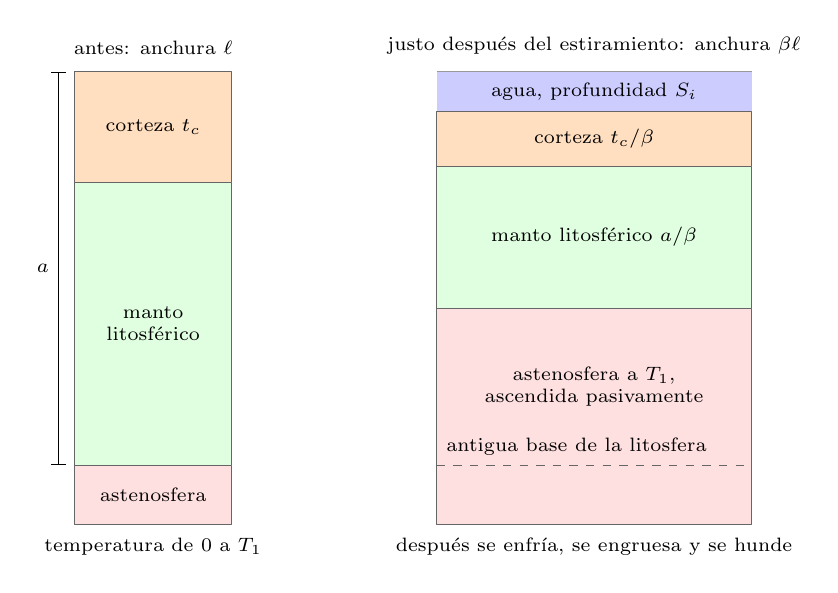
\begin{tikzpicture}[x=0.5cm, y=0.5cm, font=\scriptsize, line join=round]
% before
\begin{scope}
\fill[orange!25, draw=black!60, line width=0.3pt] (0,0) rectangle (4,-2.8);
\fill[green!12, draw=black!60, line width=0.3pt] (0,-2.8) rectangle (4,-10);
\fill[red!12, draw=black!60, line width=0.3pt] (0,-10) rectangle (4,-11.5);
\node at (2,-1.4) {corteza $t_c$};
\node[align=center] at (2,-6.4) {manto\\litosférico};
\node at (2,-10.75) {astenosfera};
\draw[|-|] (-0.4,0) -- (-0.4,-10) node[midway, left] {$a$};
\node[anchor=south] at (2,0.2) {antes: anchura $\ell$};
\node[anchor=north] at (2,-11.6) {temperatura de $0$ a $T_1$};
\end{scope}
% after
\begin{scope}[xshift=4.6cm]
\fill[blue!20] (0,0) rectangle (8,-1.0);
\fill[orange!25, draw=black!60, line width=0.3pt] (0,-1.0) rectangle (8,-2.4);
\fill[green!12, draw=black!60, line width=0.3pt] (0,-2.4) rectangle (8,-6.0);
\fill[red!12, draw=black!60, line width=0.3pt] (0,-6.0) rectangle (8,-11.5);
\draw[black!60, dashed] (0,-10) -- (8,-10);
\node at (4,-0.5) {agua, profundidad $S_i$};
\node at (4,-1.7) {corteza $t_c/\beta$};
\node at (4,-4.2) {manto litosférico $a/\beta$};
\node[align=center] at (4,-8.0) {astenosfera a $T_1$,\\ascendida pasivamente};
\node[anchor=south west] at (0,-10) {antigua base de la litosfera};
\node[anchor=south] at (4,0.2) {justo después del estiramiento: anchura $\beta\ell$};
\node[anchor=north] at (4,-11.6) {después se enfría, se engruesa y se hunde};
\draw[black!40] (0,0) -- (8,0);
\end{scope}
\end{tikzpicture}
\par\smallskip{\small El \omterm{def:b2:basins-compared:stretching}{modelo de estiramiento} (sin escala): una litosfera de espesor $a$ con una
corteza $t_c$ se estira hasta $\beta$ veces su anchura; la corteza y el manto litosférico se adelgazan en
$\beta$, la astenosfera asciende y la superficie se hunde en la \omterm{def:b2:basins-compared:stretching}{subsidencia sinrift} $S_i$ bajo el
agua. Aquí $\beta = 2$.}
\end{omfigure}

\begin{proposition}[Subsidencia en el modelo de estiramiento]\label{prop:b2:basins-compared:stretching}
Tenga una litosfera de espesor $a$, con una corteza de espesor $t_c$, una geoterma lineal desde
$0$ en la superficie hasta la temperatura $T_1$ de la astenosfera en su base; tengan la corteza y el manto
densidades $\rho_c(1 - \alpha T)$ y $\rho_m(1 - \alpha T)$, con $\alpha$ el coeficiente de dilatación
térmica. Si se estira instantáneamente en un factor $\beta$ y la cuenca se rellena de
agua de densidad $\rho_w$:
\begin{enumerate}
  \item la \omterm{def:b2:basins-compared:stretching}{subsidencia sinrift} es
  \[
    S_i = \frac{a\left(1 - \dfrac{1}{\beta}\right)\left[(\rho_m - \rho_c)\dfrac{t_c}{a}
          \left(1 - \dfrac{\alpha T_1 t_c}{2a}\right) - \dfrac{\alpha T_1 \rho_m}{2}\right]}
          {\rho_m(1 - \alpha T_1) - \rho_w};
  \]
  \item la \omterm{def:b2:basins-compared:stretching}{subsidencia posrift}, un tiempo $t$ después del estiramiento, es, hasta el primer término de una serie,
  \[
    S_t = E_0\,\frac{\beta}{\pi}\sin\frac{\pi}{\beta}\left(1 - e^{-t/\tau}\right),\qquad
    E_0 = \frac{4a\rho_m\alpha T_1}{\pi^2(\rho_m - \rho_w)},\qquad
    \tau = \frac{a^2}{\pi^2\kappa},
  \]
  donde $\kappa$ es la difusividad térmica y $\tau$ es la \emph{constante de tiempo
  térmica}\index{constante de tiempo térmica} de la litosfera.
\end{enumerate}
\end{proposition}
% ledger: pybacktrack:rifting

\begin{proof}
(1) Compárese la columna antes del estiramiento con la columna justo después, hasta la antigua base de
la litosfera, a una profundidad $a$ bajo la superficie anterior al estiramiento. Antes, la corteza de
espesor $t_c$ y el manto litosférico están a temperaturas $T = T_1 z/a$; después, ambos son
más delgados en un factor $\beta$ y sus temperaturas van de $0$ a $T_1$ en $a/\beta$, de modo que un punto
a la profundidad $z'$ bajo la base del agua tiene $T = T_1\beta z'/a$; debajo, la astenosfera a
$T_1$ tiene densidad $\rho_m(1 - \alpha T_1)$; encima, el agua rellena la profundidad $S_i$. La masa de una
capa de densidad $\rho(1 - \alpha T)$ en la que $T$ crece linealmente de $T_a$ a $T_b$ es
$\rho\,h\,(1 - \alpha(T_a + T_b)/2)$. Antes, la columna contiene
\[
  \rho_c t_c\left(1 - \frac{\alpha T_1 t_c}{2a}\right)
  + \rho_m (a - t_c)\left(1 - \frac{\alpha T_1 (a + t_c)}{2a}\right);
\]
después, contiene el agua, la corteza y el manto litosférico adelgazados, y la astenosfera que
rellena el resto de la profundidad $a$:
\[
  \rho_w S_i + \frac{\rho_c t_c}{\beta}\left(1 - \frac{\alpha T_1 t_c}{2a}\right)
  + \frac{\rho_m (a - t_c)}{\beta}\left(1 - \frac{\alpha T_1 (a + t_c)}{2a}\right)
  + \rho_m(1 - \alpha T_1)\left(a - S_i - \frac{a}{\beta}\right).
\]
La isostasia iguala ambas. Reuniendo los términos en $S_i$ en un lado y el factor
$(1 - 1/\beta)$ en el otro, y desarrollando, se obtiene la fórmula; el álgebra es el
\cref{exo:b2:basins-compared:11}.

(2) Tras el estiramiento, la placa se enfría por conducción entre una superficie mantenida a $0$ y una base mantenida
a $T_1$, hacia el perfil lineal del que partió. El exceso de temperatura satisface la ecuación del
calor con valores nulos en el techo y en la base, y es por tanto una suma de términos
$b_n\sin(n\pi z/a)\,e^{-n^2\kappa\pi^2 t/a^2}$; cada uno se enfría con su propio tiempo, $\tau/n^2$. El
calor perdido hace que la columna se contraiga en $\alpha\int \Delta T\,\mathrm{d}z$, y el agua adicional
que rellena el espacio la hunde aún más en el factor $\rho_m/(\rho_m - \rho_w)$. Solo contribuyen los términos
impares; conservar el primero, cuyo coeficiente se calcula a partir del perfil inicial, da
la expresión. Los demás se enfrían nueve o más veces más deprisa, y al cabo de unos diez millones de años
desplazan la subsidencia en una cantidad casi constante, de menos de \qty{100}{m} para $\beta$ de
1.2 a 4 con los valores siguientes.
\end{proof}
% values (script): basins.thermal_series vs basins.thermal, tested in tests/bachelor-2/test_basins.py

Los parámetros del artículo de McKenzie son $a = \qty{125}{km}$, $T_1 = \qty{1333}{\celsius}$,
$\alpha = \qty{3.28e-5}{K^{-1}}$, $\kappa = \qty{8e-7}{m^2.s^{-1}}$, $\rho_m =
\qty{3330}{kg.m^{-3}}$ (a \qty{0}{\celsius}), $\rho_c = \qty{2800}{kg.m^{-3}}$; con agua de mar a
\qty{1030}{kg.m^{-3}} dan $\tau = \qty{62.7}{Myr}$ y $E_0 = \qty{3207}{m}$. Con una corteza de
\qty{35}{km}, la \omterm{def:b2:basins-compared:stretching}{subsidencia sinrift} es $S_i = \qty{4334}{m} \times (1 - 1/\beta)$.
% ledger: sheplev98:parameters, pybacktrack:rifting
% values (script): tau_Myr 62.7, E0_m 3206.9, Si_max_m 4333.8

\begin{omfigure}
\centering
% figdata/bachelor-2/basins.py part curves
\begin{tikzpicture}
\begin{axis}[width=0.8\linewidth, height=6.2cm, y dir=reverse, xmin=0, xmax=200, ymin=0,
  ymax=6500, xlabel={tiempo tras el estiramiento (\unit{Myr})},
  ylabel={subsidencia tectónica (\unit{m})}, tick label style={font=\scriptsize},
  label style={font=\small}, xtick pos=bottom, ytick pos=left]
\addplot[black!45, line width=1pt] table[x=t_Myr, y=b1.2] {figdata/out/bachelor-2-basins-curves.dat};
\addplot[blue!70!black, line width=1pt] table[x=t_Myr, y=b1.5] {figdata/out/bachelor-2-basins-curves.dat};
\addplot[omThm, line width=1pt] table[x=t_Myr, y=b2] {figdata/out/bachelor-2-basins-curves.dat};
\addplot[orange!80!black, line width=1pt] table[x=t_Myr, y=b4] {figdata/out/bachelor-2-basins-curves.dat};
\node[font=\scriptsize, anchor=south west, inner sep=1pt] at (axis cs:150,1225) {$\beta = 1.2$};
\node[font=\scriptsize, anchor=south west, inner sep=1pt] at (axis cs:150,2595) {$\beta = 1.5$};
\node[font=\scriptsize, anchor=south west, inner sep=1pt] at (axis cs:150,3965) {$\beta = 2$};
\node[font=\scriptsize, anchor=south west, inner sep=1pt] at (axis cs:150,5815) {$\beta = 4$};
\draw[black!40, dashed] (axis cs:62.7,0) -- (axis cs:62.7,6500);
\node[font=\scriptsize, anchor=north west] at (axis cs:63,150) {$t = \tau$};
\end{axis}
\end{tikzpicture}
\par\smallskip{\small Subsidencia cargada de agua del \omterm{def:b2:basins-compared:stretching}{modelo de estiramiento} para cuatro \omterm{def:b2:basins-compared:stretching}{factores de
estiramiento}, con una corteza de \qty{35}{km} y los parámetros del texto: el salto sinrift en
$t = 0$, y después la curva posrift, que ha alcanzado el \qty{63}{\percent} de su valor final en
$t = \tau$.}
\end{omfigure}

Tres rasgos del modelo se trasladan a las cuencas reales.
\begin{itemize}
  \item El salto sinrift crece con $\beta$, y también la \omterm{def:b2:basins-compared:stretching}{subsidencia posrift}; pero su
        razón cambia poco, de modo que ambas partes apuntan al mismo $\beta$ si el modelo se cumple.
  \item La escala de tiempo de la \omterm{def:b2:basins-compared:stretching}{subsidencia posrift} no depende de $\beta$: la fija solo el
        espesor de la litosfera. Al cabo de $\tau$ se ha completado el \qty{63}{\percent} de la subsidencia
        térmica; al cabo de $3\tau$, cerca del \qty{95}{\percent}. Un rift que se detuvo hace doscientos
        millones de años apenas se hunde ya.
  \item El término sinrift es una competencia entre la corteza ligera adelgazada, que hace hundirse
        la superficie, y la astenosfera caliente ascendida, que la hace flotar. Con una corteza delgada gana
        la segunda y el estiramiento eleva la superficie (\cref{exo:b2:basins-compared:10}).
\end{itemize}

Para ajustar un sondeo, la subsidencia tectónica al final del rifting da $S_i$, y por tanto
$\beta = 1/(1 - S_i/\qty{4334}{m})$ para una corteza de \qty{35}{km}; la curva posrift se predice entonces
y se compara con el resto de los puntos obtenidos por \omterm{def:b2:basins-compared:backstripping}{backstripping}. En el sondeo inventado, $S_i = \qty{1441}{m}$
da $\beta = 1.50$, y la curva pasa a pocos metros de los puntos posteriores (figura de la
\cref{sec:b2:basins-compared:backstripping}). Las cuencas reales rara vez son tan complacientes. En el
centro del mar del Norte, un estiramiento del 50 al \qty{100}{\percent} en el centro, $\beta$ de 1.5 a 2,
reproduce la amplitud y la velocidad de la \omterm{def:b2:basins-compared:stretching}{subsidencia posrift}. En el margen del este de
Estados Unidos, solo un segmento, la plataforma de Long Island, tiene un relleno posrift temprano tan grueso
como predice el estiramiento uniforme; en la cuenca de Georges Bank y la fosa de Baltimore Canyon el
relleno es de 1.5 a 3 veces más grueso, y deben intervenir otras causas.
% ledger: sc80b4:north-sea, lang24:atlantic

\section{Cuencas comparadas}\label{sec:b2:basins-compared:compared}

La tabla siguiente reúne las cuatro familias. Las curvas difieren en forma y en escala de tiempo, y una
\omterm{def:b2:basins-compared:curve}{curva de subsidencia} es a menudo el primer indicio de la naturaleza de una cuenca enterrada bajo rocas más jóvenes.

\begin{center}
\small
\begin{tabular}{>{\raggedright\arraybackslash}p{0.13\linewidth}>{\raggedright\arraybackslash}p{0.19\linewidth}>{\raggedright\arraybackslash}p{0.26\linewidth}>{\raggedright\arraybackslash}p{0.29\linewidth}}
\hline
cuenca & ejemplo & espesor y duración & forma de la \omterm{def:b2:basins-compared:curve}{curva de subsidencia} tectónica \\
\hline
rift & centro del mar del Norte & fosas desde el Triásico; último estiramiento del Jurásico Medio a
mediados del Cretácico; 1.1 a \qty{1.4}{km} de hundimiento posrift cargado de agua & un salto sinrift rápido,
después una ralentización exponencial con $\tau$ de decenas de Myr \\
margen pasivo & fosa de Baltimore Canyon & más de \qty{14}{km} desde el Jurásico & como un
rift, con una gran parte posrift; el relleno se engruesa hacia el océano \\
antepaís & \omterm{def:b2:alpine-orogen:foreland}{Molasa} del norte de los Alpes & más de \qty{4}{km} en el frente de cabalgamiento, del Eoceno superior al
Mioceno superior & más profunda junto a la cordillera y migrando con ella; su parte interna acaba
cabalgada por los cabalgamientos \\
intracratónica & Michigan & más de \qty{4}{km} en episodios a lo largo de unos 500 Myr & lenta, con
episodios de hundimiento más rápido compartidos por cuencas lejanas \\
\hline
\end{tabular}
\end{center}
% ledger: sc80b4:north-sea, schlee76:atlantic, poag79:bct, krenmayr99:molasse, schmid04:foreland, sloss82:michigan

Una \omterm{def:b2:alpine-orogen:foreland}{cuenca de antepaís} se hunde bajo una carga que se desplaza hacia ella: la cuenca migra con la cordillera,
la alpina al menos \qty{210}{km} sobre el cratón europeo, y su parte interna acaba
cabalgada y transportada por los cabalgamientos, como lo fue la \omterm{def:b2:alpine-orogen:foreland}{Molasa} Subalpina en el
\cref{ch:b2:alpine-orogen}. Un rift se ralentiza a medida que se enfría, sea cual sea
su estiramiento. Una \omterm{def:b2:basins-compared:types}{cuenca intracratónica} se hunde lenta y prolongadamente, a impulsos; ni el estiramiento
ni una carga la explican bien, y por eso sigue siendo una cuestión de investigación.
% ledger: schmid04:foreland, sinclair97:trinity, krenmayr99:molasse

\begin{inthelab}[Análisis de la subsidencia]
Los analistas de cuencas hacen con programas el trabajo del recuadro de método. Un programa de código abierto, por
ejemplo, lee un sondeo como una lista de unidades con sus edades, profundidades y litologías, y una
tabla de litologías con su densidad de grano, su porosidad superficial y su longitud de decaimiento. Su
módulo de \omterm{def:b2:basins-compared:backstripping}{backstripping} descompacta las unidades y devuelve la subsidencia tectónica en cada edad;
como la paleoprofundidad del agua solo se conoce como un intervalo, el usuario da un mínimo y un máximo y
el programa devuelve las dos subsidencias y su media. Un segundo módulo trabaja en sentido inverso:
a partir de un modelo de subsidencia tectónica predice las profundidades de agua del pasado, que pueden
contrastarse con los fósiles. Los analistas ajustan después \omterm{def:b2:basins-compared:stretching}{factores de estiramiento}, ponen a prueba curvas del nivel del mar y
cartografían la subsidencia de toda una cuenca a partir de cientos o miles de sondeos.
\end{inthelab}
% ledger: pybacktrack:modules, crowe09:michigan

\section*{Ejercicios}\label{sec:b2:basins-compared:exercises}

Datos para los ejercicios, salvo indicación contraria: $\rho_m = \qty{3330}{kg.m^{-3}}$, $\rho_c =
\qty{2800}{kg.m^{-3}}$, $\rho_w = \qty{1030}{kg.m^{-3}}$; \omterm{def:b2:basins-compared:stretching}{modelo de estiramiento} con $a =
\qty{125}{km}$, $T_1 = \qty{1333}{\celsius}$, $\alpha = \qty{3.28e-5}{K^{-1}}$, $\kappa =
\qty{8e-7}{m^2.s^{-1}}$, $\tau = \qty{62.7}{Myr}$, $E_0 = \qty{3207}{m}$; una corteza de \qty{35}{km}
da $S_i = \qty{4334}{m}\times(1 - 1/\beta)$; constantes litológicas en la tabla de la
\cref{sec:b2:basins-compared:curves}.

\begin{exercise}[$\star$]\label{exo:b2:basins-compared:1}
Nómbrense la familia de cada cuenca y la causa principal de su subsidencia: (a) la cuenca de Michigan;
(b) el centro del mar del Norte; (c) la fosa de Baltimore Canyon; (d) la \omterm{def:b2:alpine-orogen:foreland}{Molasa} del norte de los Alpes;
(e) la llanura indogangética delante del Himalaya.
\end{exercise}

\begin{exercise}[$\star$]\label{exo:b2:basins-compared:2}
Una cuenca contiene \qty{3.0}{km} de sedimento de densidad media \qty{2300}{kg.m^{-3}}. (a) Hállese su
subsidencia tectónica si el sedimento llega al nivel del mar. (b) ¿Y si hay \qty{200}{m} de agua
encima? (c) ¿Qué fracción del espesor del relleno se debe a la carga del propio relleno?
\end{exercise}

\begin{exercise}[$\star$]\label{exo:b2:basins-compared:3}
La sísmica de refracción muestra que una corteza de \qty{35}{km} se ha adelgazado hasta \qty{25}{km} en un rift.
(a) ¿Cuánto vale $\beta$? (b) ¿Qué espesor tiene la litosfera justo después del estiramiento? (c) ¿Cuál es la
\omterm{def:b2:basins-compared:stretching}{subsidencia sinrift} bajo agua?
\end{exercise}

\begin{exercise}[$\star$]\label{exo:b2:basins-compared:4}
(a) Compruébese que $\tau = \qty{62.7}{Myr}$ ($1~\text{Myr} = \qty{3.156e13}{s}$). (b) Algunos programas
usan $\kappa = \qty{1e-6}{m^2.s^{-1}}$: ¿cuánto vale entonces $\tau$? (c) ¿Cuánto valdría para una
litosfera de \qty{100}{km} de espesor, con $\kappa = \qty{8e-7}{m^2.s^{-1}}$? (d) ¿Qué fracción de
la \omterm{def:b2:basins-compared:stretching}{subsidencia posrift} se ha completado al cabo de $\tau$, y al cabo de $3\tau$?
\end{exercise}

\begin{exercise}[$\star\star$]\label{exo:b2:basins-compared:5}
Una unidad de lutita se encuentra hoy entre \qty{1000}{m} y \qty{2000}{m}. (a) Hállese su porosidad en el
techo y en la base. (b) Hállese su espesor sólido. (c) Hállense su masa por unidad de área y su densidad
media, con los poros llenos de agua.
\end{exercise}

\begin{exercise}[$\star\star$]\label{exo:b2:basins-compared:6}
La lutita del \cref{exo:b2:basins-compared:5} se devuelve a la superficie. (a) Itérese la
fórmula de descompactación desde $z_2' = T_s$ hasta que cambie menos de \qty{1}{m}. (b) ¿Cuál es
su densidad media en superficie? (c) ¿Cuánto más gruesa era?
\end{exercise}

\begin{exercise}[$\star\star$]\label{exo:b2:basins-compared:7}
En el centro del mar del Norte, el basamento cargado de agua se hundió de 1100 a \qty{1400}{m} después del
estiramiento que terminó a mediados del Cretácico, hace unos \qty{100}{Myr}. (a) ¿Qué \omterm{def:b2:basins-compared:stretching}{subsidencia posrift}
da el modelo al cabo de \qty{100}{Myr} para $\beta = 1.5$ y $\beta = 2$? (b) ¿Encuadran esos
valores la observación? (c) ¿Para qué $\beta$ da el modelo \qty{1250}{m}?
Úsese $\frac{\beta}{\pi}\sin\frac{\pi}{\beta} = 0.4705$ para $\beta = 1.6$ y $0.5204$ para $\beta
= 1.7$, e interpólese.
\end{exercise}

\begin{exercise}[$\star\star$]\label{exo:b2:basins-compared:8}
La cuenca sinrift de un \omterm{def:b2:basins-compared:stretching}{modelo de estiramiento} no se rellena de agua sino de sedimento de densidad
\qty{2300}{kg.m^{-3}}. (a) En la fórmula de $S_i$, ¿qué cambia? (b) Calcúlese el $S_i$ cargado de sedimento
para $\beta = 1.5$ con una corteza de \qty{35}{km}, sabiendo que el numerador de la fórmula es
$a(1 - 1/\beta)\times\qty{74.69}{kg.m^{-3}}$ y que $\rho_m(1 - \alpha T_1) =
\qty{3184.4}{kg.m^{-3}}$. (c) Compárese con el valor cargado de agua.
\end{exercise}

\begin{exercise}[$\star\star$]\label{exo:b2:basins-compared:9}
Un sondeo sometido a \omterm{def:b2:basins-compared:backstripping}{backstripping} da $Y = \qty{2171}{m}$ a \qty{100}{Ma}, suponiendo el nivel del mar actual. (a)
Si el mar estaba entonces \qty{100}{m} más alto, ¿cuánto vale $Y$? (b) Si los fósiles dan una profundidad de agua
entre 100 y \qty{500}{m} en lugar de \qty{300}{m}, ¿qué intervalo de $Y$ resulta? (c) ¿Cuál de las
dos incertidumbres es mayor?
\end{exercise}

\begin{exercise}[$\star\star\star$]\label{exo:b2:basins-compared:10}
(a) Demuéstrese a partir de la \cref{prop:b2:basins-compared:stretching} que el estiramiento hace que la superficie se eleve
en lugar de hundirse cuando $(\rho_m - \rho_c)\frac{t_c}{a}\left(1 - \frac{\alpha T_1 t_c}{2a}\right) <
\frac{\alpha T_1\rho_m}{2}$. (b) Despreciando el término pequeño $\alpha T_1 t_c/(2a)$, hállese el
espesor cortical crítico. (c) Afínese con una iteración. (d) ¿En qué lugares de la Tierra buscaría usted
rifts que se elevan al abrirse?
\end{exercise}

\begin{exercise}[$\star\star\star$]\label{exo:b2:basins-compared:11}
(a) Escríbase el equilibrio isostático de la demostración de la \cref{prop:b2:basins-compared:stretching}, parte
(1), y dedúzcase la fórmula de $S_i$. (b) Demuéstrese que la \omterm{def:b2:basins-compared:stretching}{subsidencia posrift} final exacta, cuando
la placa ha vuelto a su geoterma lineal, es $\alpha\rho_m T_1 a(1 - 1/\beta)/(2(\rho_m -
\rho_w))$. (c) Calcúlese para $\beta = 2$ y compárese con el valor final de la
fórmula del primer término.
\end{exercise}

\begin{exercise}[$\star\star\star$]\label{exo:b2:basins-compared:12}
Un margen pasivo se estiró en un factor $\beta = 2$ y lleva \qty{150}{Myr} enfriándose; la
cuenca ha permanecido llena de sedimento de densidad media \qty{2400}{kg.m^{-3}} hasta el nivel del mar.
(a) Hállese la \omterm{def:b2:basins-compared:stretching}{subsidencia posrift} cargada de agua. (b) ¿Qué espesor tiene el sedimento posrift?
(c) En la fosa de Baltimore Canyon el relleno posrift temprano es de 1.5 a 3 veces más grueso de lo que
predice el estiramiento uniforme: ¿qué espesor supondría eso aquí? (d) Propónganse causas.
\end{exercise}

\begin{problem}[{Problema de fin de semana --- Backstripping de un sondeo}]\label{pb:b2:basins-compared:1}
En la cuenca inventada de Kestrel, un sondeo testificó cuatro unidades. Desde la base: una arena depositada durante
el rifting, de 165 a \qty{150}{Ma}, hoy entre \qty{4420}{m} y \qty{6030}{m}; una lutita, de 150
a \qty{100}{Ma}, entre \qty{3310}{m} y \qty{4420}{m}; una creta, de 100 a \qty{60}{Ma}, entre
\qty{1700}{m} y \qty{3310}{m}; una arena lutítica, de \qty{60}{Ma} a hoy, entre \qty{0}{m} y
\qty{1700}{m} bajo el fondo marino. Los fósiles dan la profundidad del agua en el techo de cada unidad cuando se
depositó: \qty{200}{m} a \qty{150}{Ma}, \qty{300}{m} a \qty{100}{Ma}, \qty{150}{m} a
\qty{60}{Ma}; hoy es de \qty{100}{m}. Úsense la tabla de litologías del capítulo, $\rho_m =
\qty{3330}{kg.m^{-3}}$ y $\rho_w = \qty{1030}{kg.m^{-3}}$ tanto para el agua de mar como para el agua intersticial, el nivel del mar
actual, y el \omterm{def:b2:basins-compared:stretching}{modelo de estiramiento} del capítulo con una corteza de \qty{35}{km}. Las profundidades se redondean
al metro.

\noindent\textbf{Parte I --- Compactación.}
\begin{enumerate}
  \item Hállese la porosidad de la arena hoy en su techo y en su base.
  \item Hállese el espesor sólido de la arena.
  \item Los espesores sólidos de la lutita, la creta y la arena lutítica son \qty{1011}{m},
        \qty{1409}{m} y \qty{1004}{m}. Compruébese uno de ellos.
  \item Hállese la masa por unidad de área de cada unidad hoy, y después la densidad media de toda la
        columna.
  \item A \qty{150}{Ma} la arena estaba en el fondo marino. Descompáctese: itérese desde $z_2' =
        T_s$ hasta que el cambio sea menor de \qty{1}{m}.
  \item Hállese la densidad media de la arena descompactada.
\end{enumerate}

\noindent\textbf{Parte II --- Backstripping.}
\begin{enumerate}[resume]
  \item Hállese la subsidencia tectónica $Y$ a \qty{150}{Ma}.
  \item Hállese la subsidencia tectónica actual. ¿Por qué no hace falta descompactar?
  \item Un programa da $Y = \qty{2171}{m}$ a \qty{100}{Ma} e $Y = \qty{2453}{m}$ a
        \qty{60}{Ma}. Calcúlese la velocidad media de subsidencia tectónica en cada uno de los tres
        intervalos desde \qty{150}{Ma}.
  \item Hállese la subsidencia total actual y compárese con la subsidencia tectónica.
  \item ¿Qué fracción de la profundidad actual del basamento se debe a la carga del sedimento?
  \item Si a \qty{100}{Ma} el mar hubiera estado \qty{100}{m} más alto que hoy, ¿cuánto habría valido
        entonces $Y$?
\end{enumerate}

\noindent\textbf{Parte III --- Ajuste del modelo de estiramiento.} El rifting se considera instantáneo
y terminado a \qty{150}{Ma}.
\begin{enumerate}[resume]
  \item ¿Qué punto de la curva da la \omterm{def:b2:basins-compared:stretching}{subsidencia sinrift}?
  \item Hállese el \omterm{def:b2:basins-compared:stretching}{factor de estiramiento} $\beta$, con dos decimales.
  \item ¿Qué espesor tenían la corteza y la litosfera justo después del estiramiento?
  \item Con $\beta$ redondeado, calcúlense $\frac{\beta}{\pi}\sin\frac{\pi}{\beta}$ y la \omterm{def:b2:basins-compared:stretching}{subsidencia
        posrift} final.
  \item Predígase $Y$ a 100, 60 y \qty{0}{Ma}.
  \item Compárese con los valores obtenidos por \omterm{def:b2:basins-compared:backstripping}{backstripping}.
  \item El ajuste es bueno porque el sondeo es inventado. Dense tres razones por las que un sondeo real
        no se ajustaría tan bien.
\end{enumerate}

\noindent\textbf{Parte IV --- Los próximos 50 millones de años.}
\begin{enumerate}[resume]
  \item ¿Cuánta subsidencia tectónica más se producirá en los próximos \qty{50}{Myr}?
  \item Si la profundidad del agua se mantiene en \qty{100}{m}, ¿cuánto sedimento de densidad
        \qty{2400}{kg.m^{-3}} puede acumularse en ese tiempo?
  \item ¿Qué fracción de su \omterm{def:b2:basins-compared:stretching}{subsidencia posrift} final ha completado ya la cuenca?
  \item ¿Cuándo se había completado la mitad?
  \item En resumen: ¿qué \omterm{def:b2:basins-compared:stretching}{factor de estiramiento} registra el sondeo?
\end{enumerate}
\end{problem}
